\documentclass[12pt, a4paper]{report}
\usepackage{graphicx} %LaTeX package to import graphics
\usepackage[shortlabels]{enumitem}
\usepackage{geometry}
\usepackage{xcolor}
\geometry{lmargin=30mm}
\usepackage[export]{adjustbox}
\usepackage{titlesec}
\usepackage{float}
\usepackage{listings}

\usepackage{hyperref}

\titleformat{\chapter}{\normalfont\huge}{\thechapter}{20pt}{\huge\bf}
\graphicspath{{images/}} %configuring the graphicx package
\title{Practica 7}
\author{Javier Izquierdo Hernández}
\date{\today}
\begin{document}
	\begin{titlepage}
		\centering
		{
\includegraphics[width=0.3\textwidth]{logo}\par}
		\vspace{1cm}
		{\bfseries\LARGE Universidad Rey Juan Carlos \par}
		\vspace{1cm}
		{\scshape\Large E.T.S. Ingeniería de Telecomunicación \par}
		\vspace{3cm}
		{\scshape\Huge Redes de Ordenadores para Robots y Máquinas Inteligentes \par}
		\vspace{3cm}
		{\itshape\Large Práctica 7\par}
		\vfill
		{\Large Autor: \par}
		{\Large Javier Izquierdo Hernández \par}
		\vfill
		{\Large \today \par}
	\end{titlepage}

\newpage
\renewcommand{\contentsname}{Contenidos}
\tableofcontents
\newpage

\chapter{Consideraciones iniciales}
Para realizar esta práctica se necesita utilizar software mqttx que actúe como servidor mqttx.
Tienes 2 opciones: 1. Puedes instalar el software mqttx en una máquina virtual con Ubuntu. Continúa
en el paso 2.\\

2. Puedes utilizar el software mqttx instalado en los laboratorios. Continúa en el paso 3.

\chapter{Usuarios con linux en su PC o utilizando una imagen}
Importante: usuarios que utilicen su propio PC con Linux o tengan una imagen como la proporcio-
nada aqui https://labs.etsit.urjc.es/index.php/tutoriales/imagenes-ubuntu-virtualbox/
\section{Instalación de mqttx}
Instala la siguiente aplicación que será un cliente mqtt. Se utilizará la aplicación mqttx,
https://mqttx.app/. La instalación en ubuntu se realiza ejecutando los siguientes comandos:\\
\begin{center}
	sudo apt update\\
	sudo apt install snapd\\
	sudo snap install mqttx
\end{center}
Si lo instaláis usando la interfaz gráfica se mostrará una pantalla como esta
\begin{figure}[H]
	\centering
	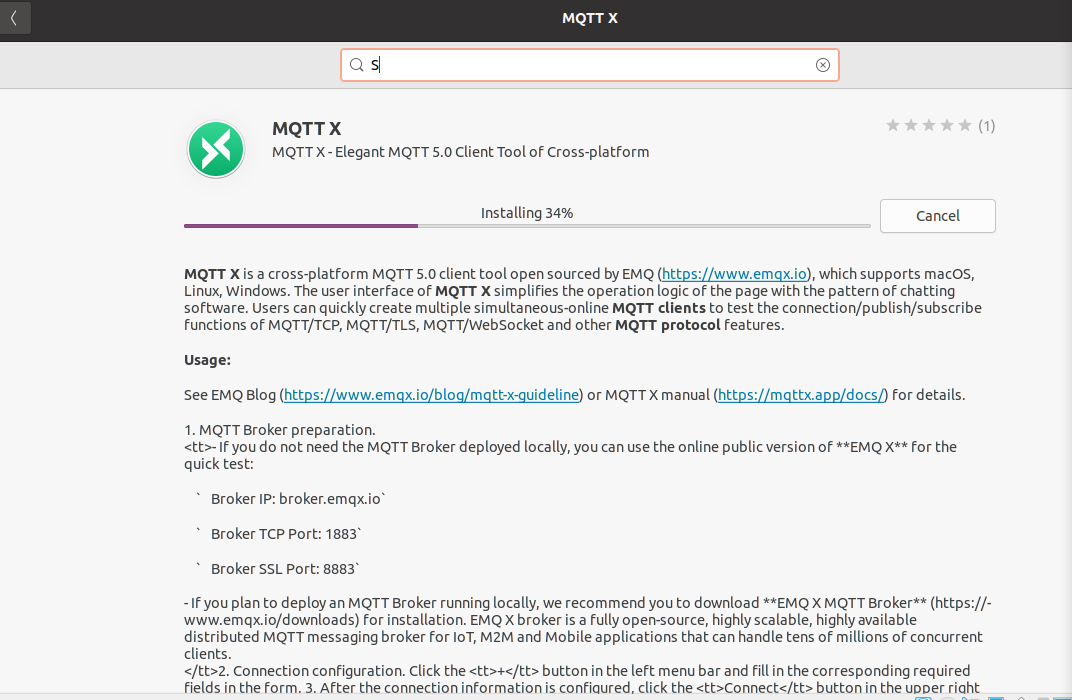
\includegraphics[width=0.8\textwidth]{enun1}
\end{figure}
Una vez instalada, se puede ejecutar de la siguiente forma:
\begin{figure}[H]
	\centering
	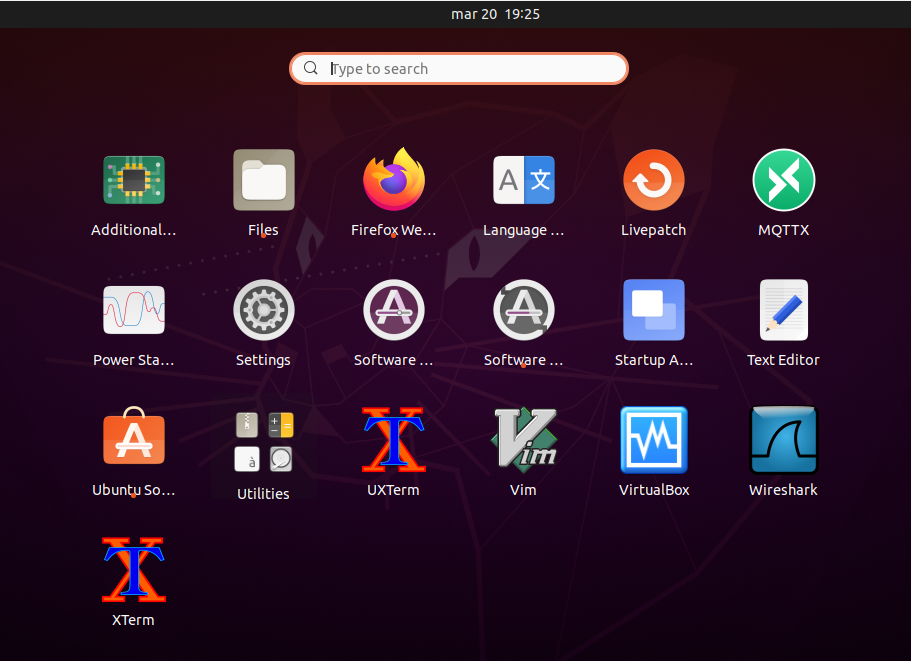
\includegraphics[width=0.8\textwidth]{enun2}
\end{figure}
\textbf{Importante}: En esta práctica, el consumidor y el productor están en el mismo host (vuestro
ordenador) que ejecuta el cliente mqtt con el software (mqtttx)
\begin{figure}[H]
	\centering
	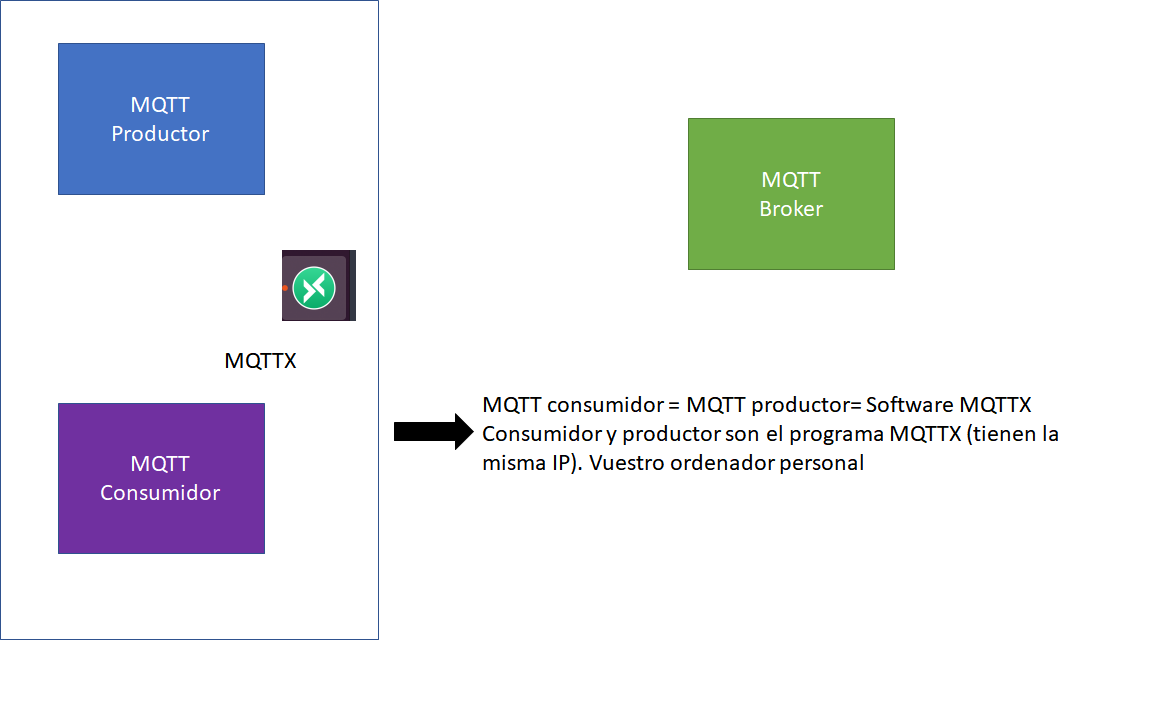
\includegraphics[width=0.8\textwidth]{enun3}
\end{figure}
Continúa en el paso 4
\chapter{Usuarios con vncweb o usuarios en los laboratorios}
Conectate con tu usuario al laboratorio https://labs.eif.urjc.es/vnc/ o en el pc de los laboratorios
\section{Uso de mqttx}
Usa la aplicación instalada
\begin{figure}[H]
	\centering
	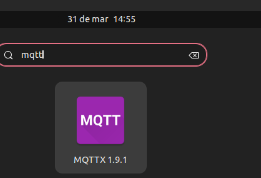
\includegraphics[width=0.8\textwidth]{enun4}
\end{figure}
\textbf{Importante}: En esta práctica, el consumidor y el productor están en el mismo host (vuestro ordenador)
que ejecuta el cliente mqtt con el software (mqtttx)
\begin{figure}[H]
	\centering
	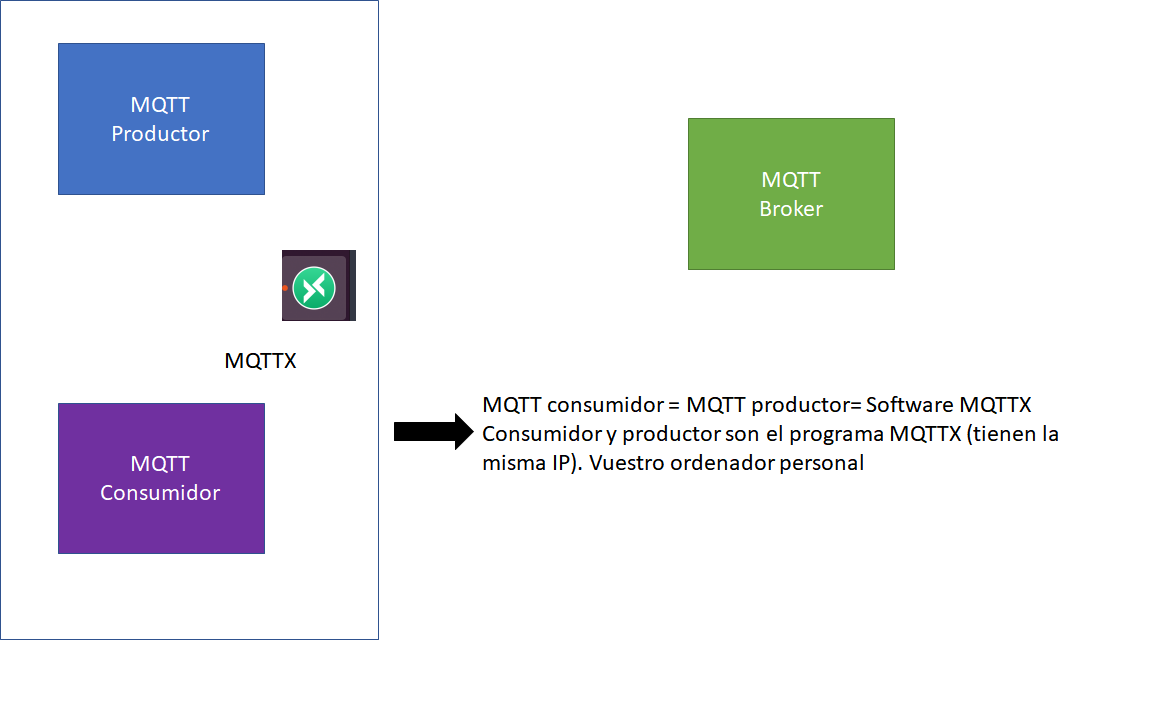
\includegraphics[width=0.8\textwidth]{enun5}
\end{figure}
\chapter{Connect}
\begin{enumerate}
	\item En un terminal ejecuta el siguiente comando para lanzar una captura de tráfico.
	\begin{center}
		sudo tcpdump -i any -s 0 -w mqtt-01.cap
	\end{center}
	Nota: Puedes capturar paquetes también con wireshark seleccionando any como la interfaz que
	quieres capturar. Para ello tienes que haber instalado wireshark con permisos para que cualquier
	usuario pueda capturar tráfico, o deberás lanzar wireshark con sudo.
	\item Crea una nueva conexión
	\begin{figure}[H]
		\centering
		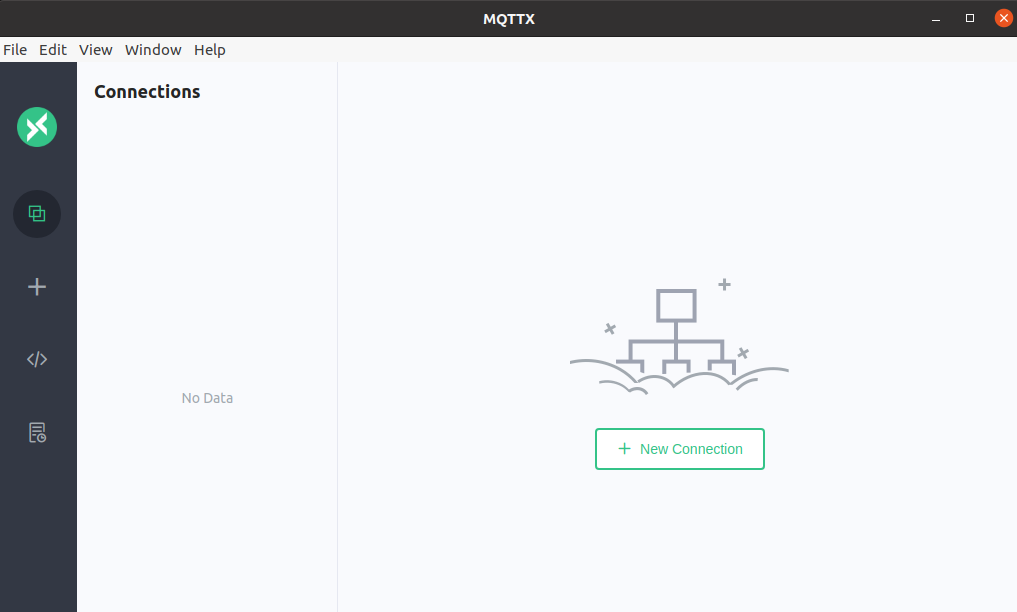
\includegraphics[width=0.8\textwidth]{enun6}
	\end{figure}
	Con las siguientes propiedades
	\begin{center}
		Name: test.mosquitto.org
		Host: test.mosquitto.org
		Port:1883
	\end{center}
	\begin{figure}[H]
		\centering
		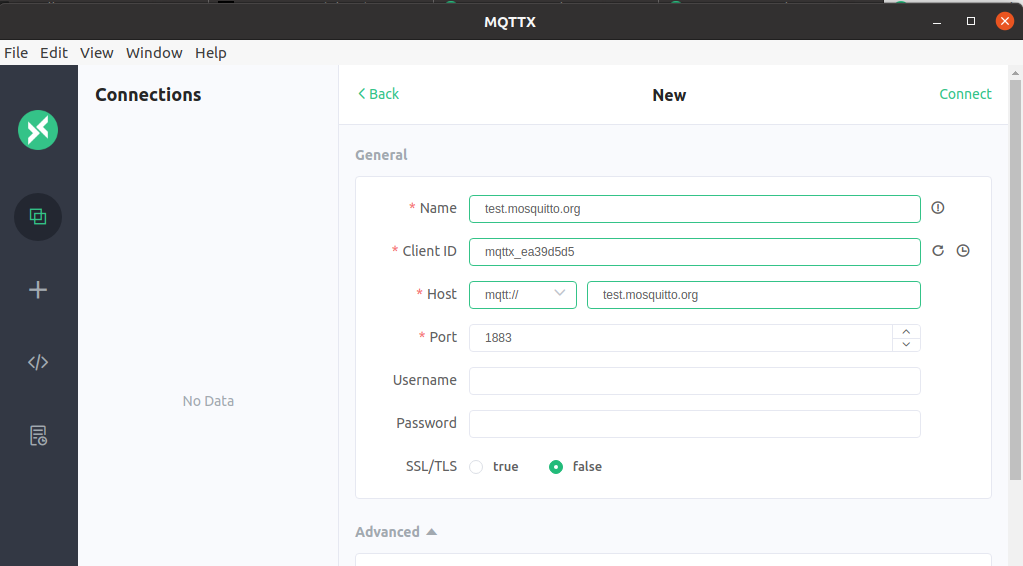
\includegraphics[width=0.8\textwidth]{enun7}
	\end{figure}
	\item Conectate usando el botón del navegador Connect (arriba a la derecha)
	\begin{figure}[H]
		\centering
		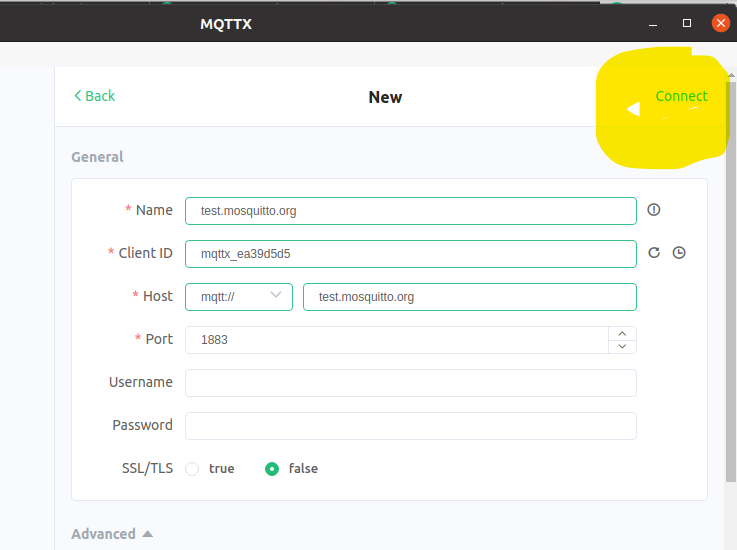
\includegraphics[width=0.8\textwidth]{enun8}
	\end{figure}
	Verifica que la versión es 3.1 y que el auto reconnect está deshabilitado. Este menú esta disponible
	en la parte Advanced de la configuración del sevidor
	\begin{figure}[H]
		\centering
		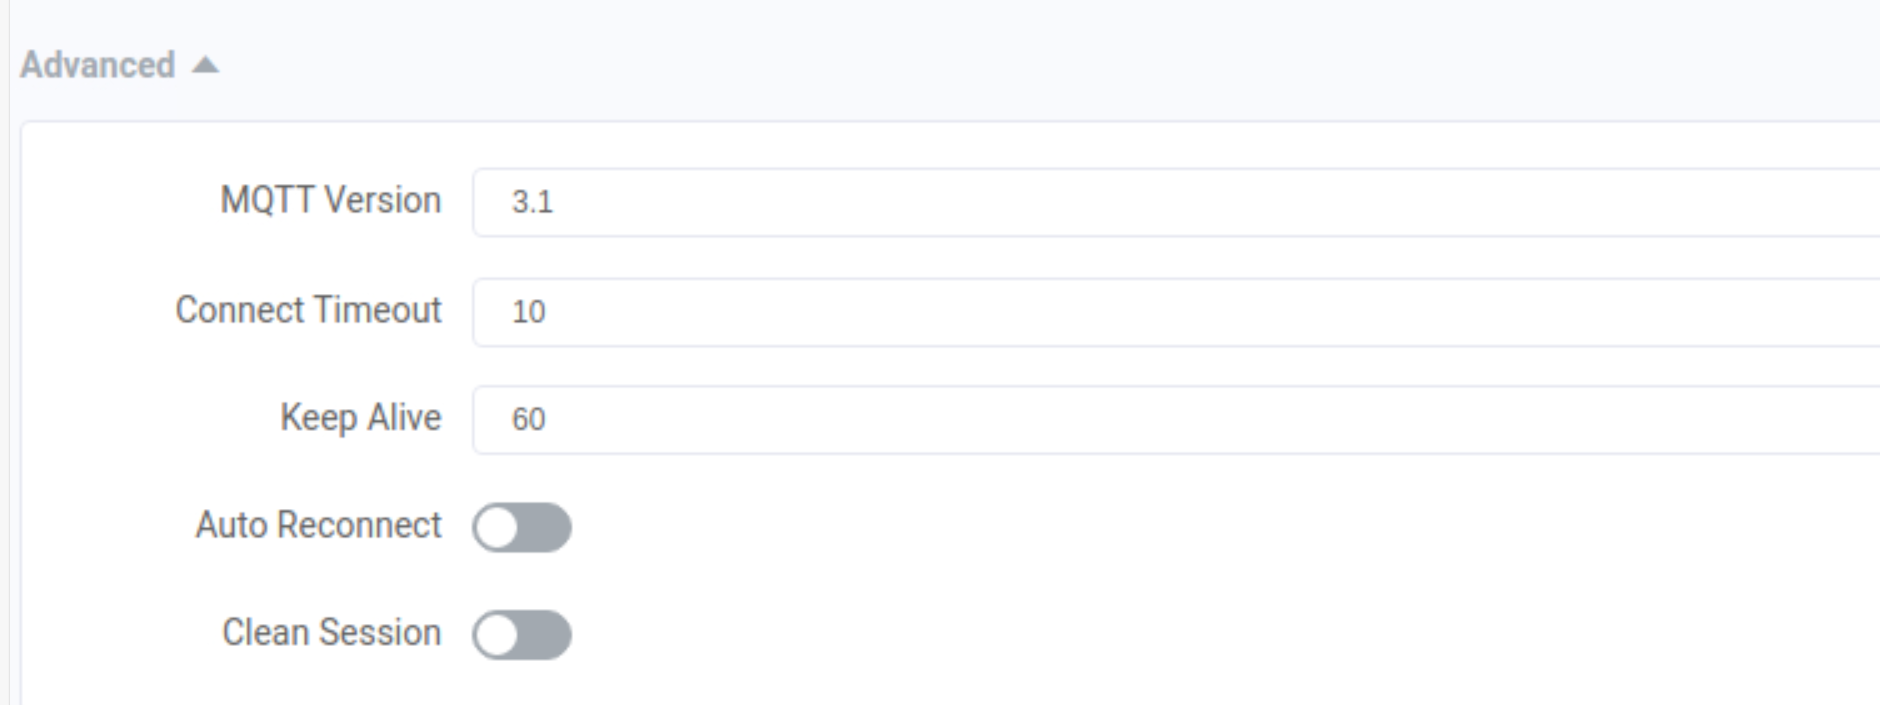
\includegraphics[width=0.8\textwidth]{enun9}
	\end{figure}
	La conexión se pondrá en verde:
	\begin{figure}[H]
		\centering
		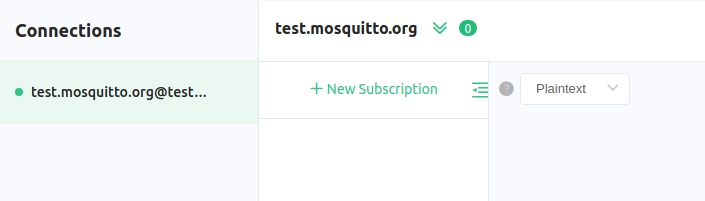
\includegraphics[width=0.8\textwidth]{enun10}
	\end{figure}
	\item Para la captura con Control+C.
	\item Abre la captura en wireshark. Si no tienes permisos para abrir la captura, cámbiaselos con
	sudo chmod.\\
	La conexión de este MQTT cliente se realiza utilizando el puerto 1883. En algunas versiones de
	wirehark no se identifica automáticamente el protocolo MQTT. Si te ocurre así, localiza en la
	captura los paquetes que tienen el puerto 1883, por ejemplo con el filtro tcp.port==1883
	\begin{figure}[H]
		\centering
		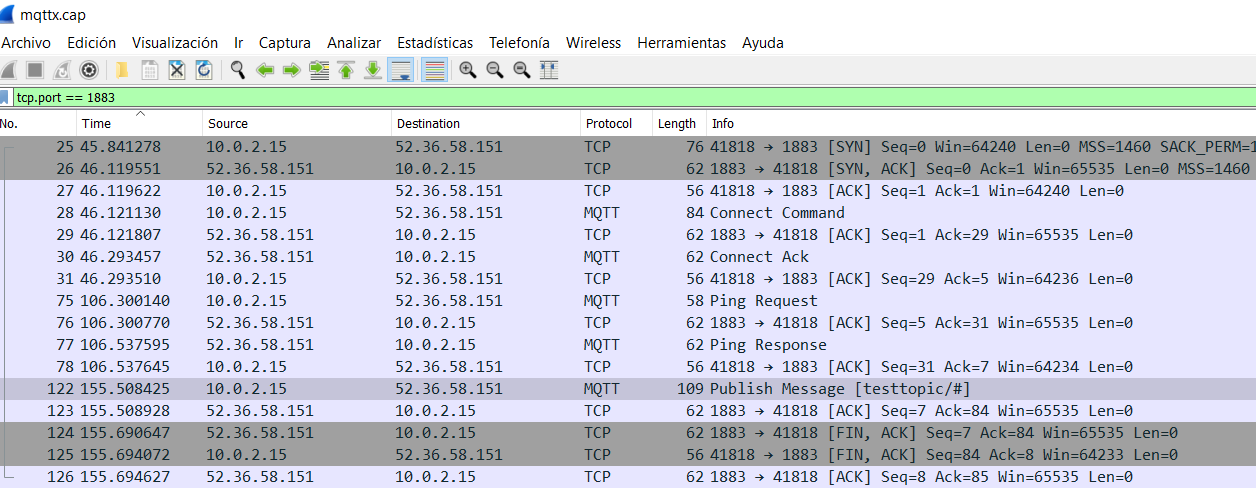
\includegraphics[width=0.8\textwidth]{enun11}
	\end{figure}
	Selecciona uno de los mensajes y haciendo click con el botón derecho, Selecciona Decode as...:
	\begin{figure}[H]
		\centering
		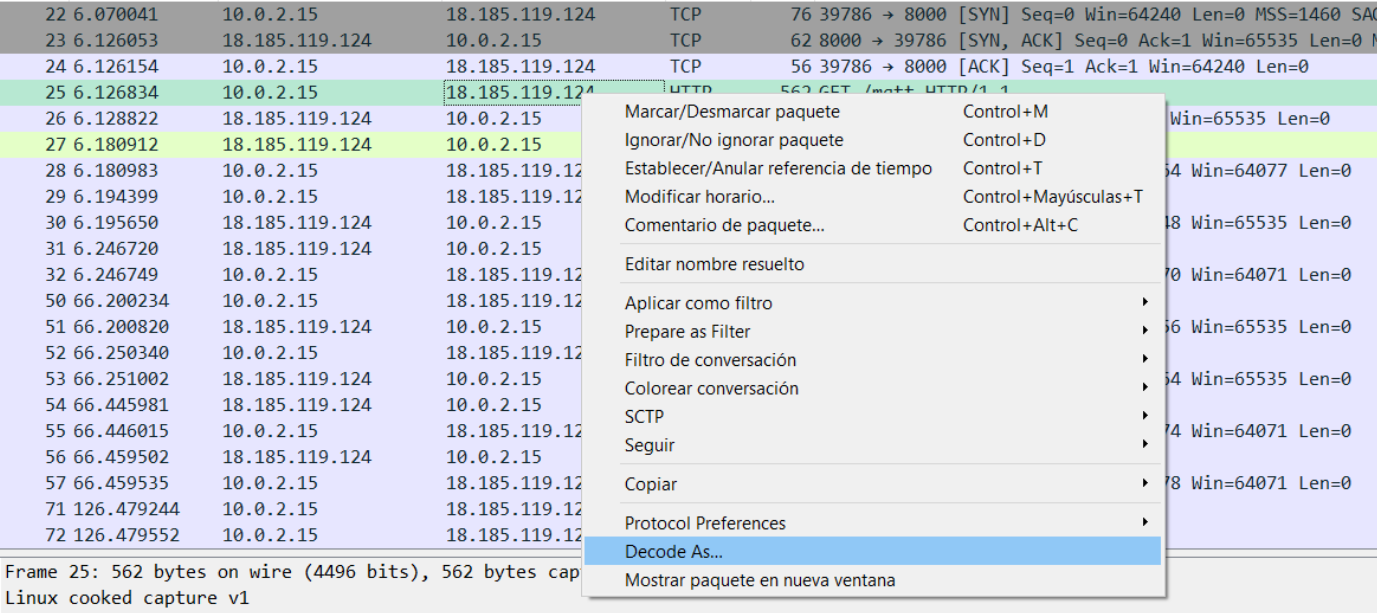
\includegraphics[width=0.8\textwidth]{enun12}
	\end{figure}
	Posteriormente indica que el protocolo será MQTT:
	\begin{figure}[H]
		\centering
		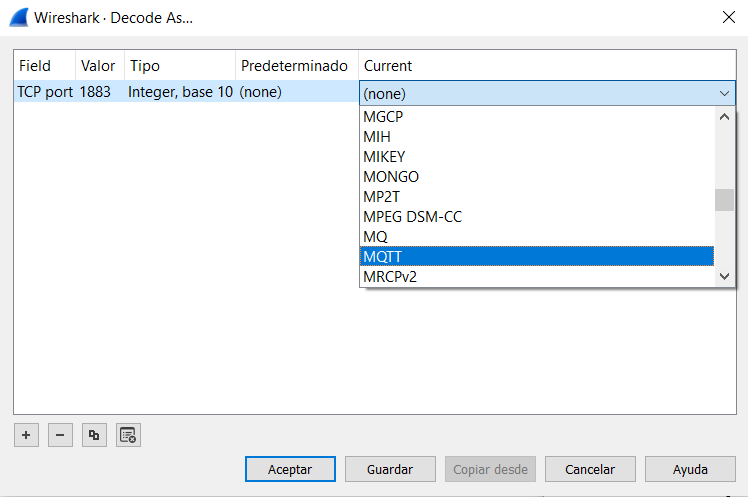
\includegraphics[width=0.8\textwidth]{enun13}
	\end{figure}
	Una vez que wireshark identifica correctamente los paquetes del protocolo MQTT, para seleccionar los paquetes en la captura puedes usar simplemente un filtro con el nombre del protocolo:
	mqtt.\\
	Identifica el mensaje \textbf{Connect}.
	\begin{figure}[H]
		\centering
		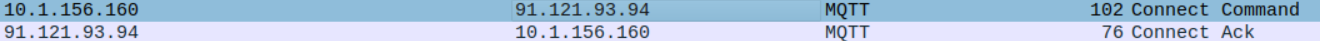
\includegraphics[width=0.8\textwidth]{ej4.5}
	\end{figure}
	\item ¿Qué dirección IP utiliza el cliente MQTT?\\
	
	10.1.156.160
	\item ¿Qué dirección IP utiliza el broker?\\
	
	91.121.93.94
	\item ¿Qué versión se utiliza del protocolo MQTT?\\
	
	v3.1
	\item ¿Qué client id utiliza?\\
	
	mqttx\_4964f260
	\item En el mensaje de Connection Ack, ¿qué código devuelve? ¿qué significa ese código?\\
	
	Devuelve el código 0 que significa conexión aceptada.
	\item ¿Tiene el parámetro Clean Session activo?\\
	
	No
\end{enumerate}
\chapter{Ping}
\begin{enumerate}
	\item Ponte a capturar tráfico en el fichero \textcolor{blue}{mqtt-02.cap}.
	\item Verifica que la conexión está activa. Deja 3 minutos la captura.
	\item Para la captura con Control+C.
	\item Abre la captura en wireshark. Identifica los mensajes Ping
	\item ¿Cada cuánto tiempo se producen los mensajes Ping? ¿Dónde has configurado ese valor? ¿Dónde
	lo puedes observar? Pista: Chequea los mensajes connect del apartado anterior\\
	
	Se mandan cada 60 segundos o 1 minuto, y esto esta configurado en el campo Keep Alive que tiene un valor de 60, es decir que la conexión se restaura cada 60 segundos al mandar el ping para comprobar si todo sigue igual.\\
	\begin{figure}[H]
		\centering
		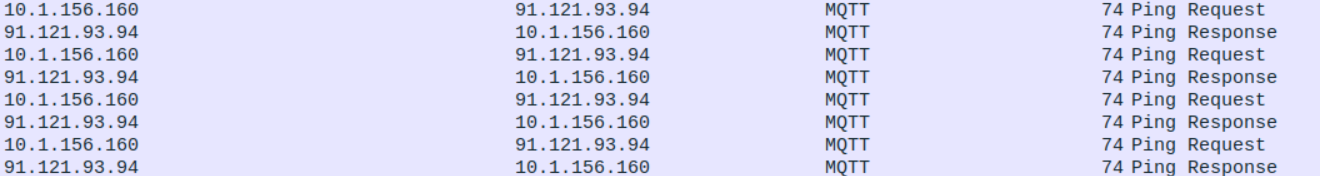
\includegraphics[width=0.8\textwidth]{ej5.4}
	\end{figure}
	\item ¿Qué longitud de mensaje tiene el ping request?\\
	
	0 bytes.
	\item ¿Qué longitud de mensaje tiene el ping response?\\
	
	0 bytes.
\end{enumerate}
\chapter{Subscribe}
\begin{enumerate}
	\item Ponte a capturar tráfico en el fichero \textcolor{blue}{mqtt-03.cap}.
	\item Verifica que la conexión está activa.
	\item Subscribe tu cliente (consumidor) al siguiente tema con Qos 0.\\
	\textbf{IMPORTANTE: Utiliza como X el valor que tienen tus direcciones IP en los escenarios de red las prácticas, como por ejemplo, el segundo byte de las direcciones IP
		en la práctica 4:}
	\begin{center}
		testtopic/p7/X/Qos0
	\end{center}
	\item Subscribe tu cliente (consumidor) al siguiente tema con Qos 1. Asegúrate de ajustar el campo
	QoS de la subscripción.
	\begin{center}
		testtopic/p7/X/Qos1
	\end{center}
	\item Subscribe tu cliente (consumidor) al siguiente tema con Qos 2. Asegúrate de ajustar el campo
	QoS de la subscripción.
	\begin{center}
		testtopic/p7/X/Qos2
	\end{center}
	\item Para la captura con Control+C.
	\item Abre la captura en wireshark. Identifica los mensajes \textbf{Subscribe}
	\item ¿A qué topics te has subscrito?\\
	
	Me he subscrito a testtopic/p7/209/Qos0, testtopic/p7/209/Qos1, testtopic/p7/209/Qos2.
	\item Identifica los diferentes mensaje de subscripción por tu cliente como Qos=0, Qos=1, Qos=2
	¿cómo los has reconocido?\\
	Chequéalo identificando el contenido del mensaje.\\
	
	Por el campo Requested QoS
	\begin{figure}[H]
		\centering
		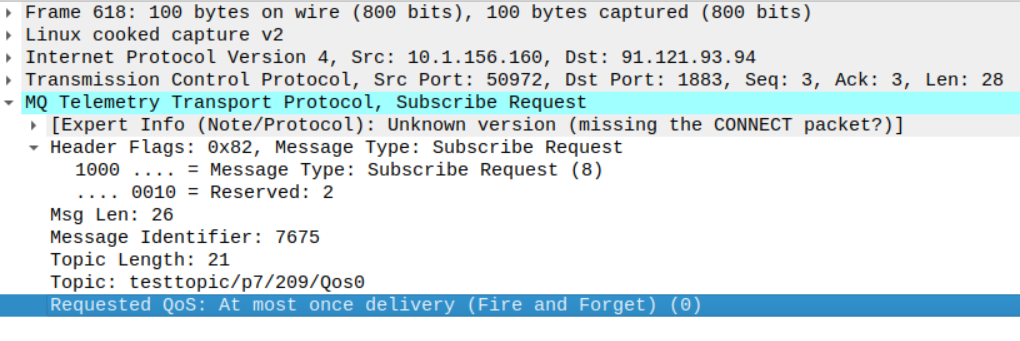
\includegraphics[width=0.8\textwidth]{ej6.9}
	\end{figure}
	\item ¿Quién es el originante (productor del mensaje)? ¿Cliente o Broker?\\
	
	El orginante de los mensajes de subscripción es el cliente. 
	\item Identifica los mensajes Subscribe Ack. ¿Qué campo utiliza para identificar el topic del Subscribe
	Request en cada uno de los mensajes ¿Cuántos mensajes Subscribe tienes? ¿Cuántos mensajes
	Subscribe Ack?\\
	
	Los mensajes de Subscribe Ack usan el campo message identifier para saber que mensaje contiene el topic que aceptan.\\
	
	Por último, como hay 3 Subscribe hay 3 Ack.
	
\end{enumerate}
\chapter{Publish}
\begin{enumerate}
	\item Elimina las subscripciones del apartado anterior:
	\begin{figure}[H]
		\centering
		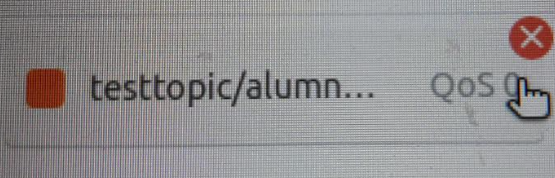
\includegraphics[width=0.4\textwidth]{enun14}
	\end{figure}
	\item Ponte a capturar tráfico en el fichero \textcolor{blue}{mqtt-04.cap}.
	\item Verifica que la conexión está activa.
	\item Publica un mensaje con Qos 0 con el topic testtopic/p7/X. Incluye en el texto del mensaje
	Qos 0
	\begin{figure}[H]
		\centering
		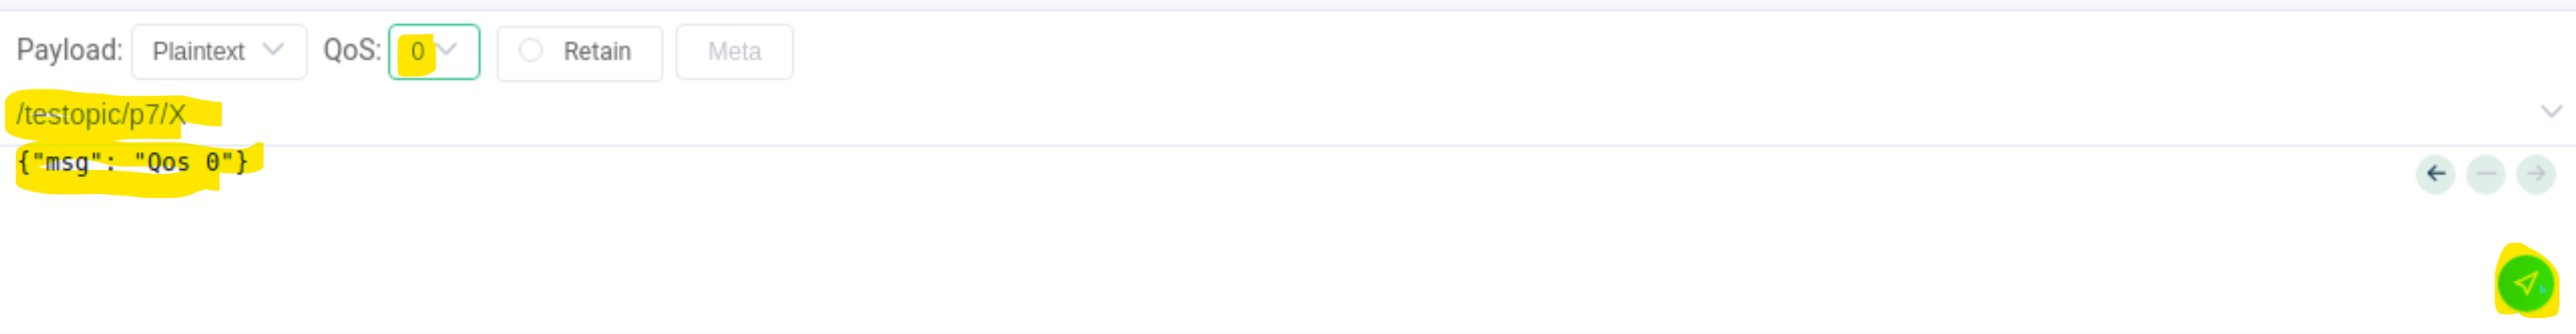
\includegraphics[width=0.8\textwidth]{enun15}
	\end{figure}
	NOTA: Verás aparecer los mensajes que publicas justo encima de donde los escribes. También
	puedes comprobar el comportamiento del cliente en el panel de log:
	\begin{figure}[H]
		\centering
		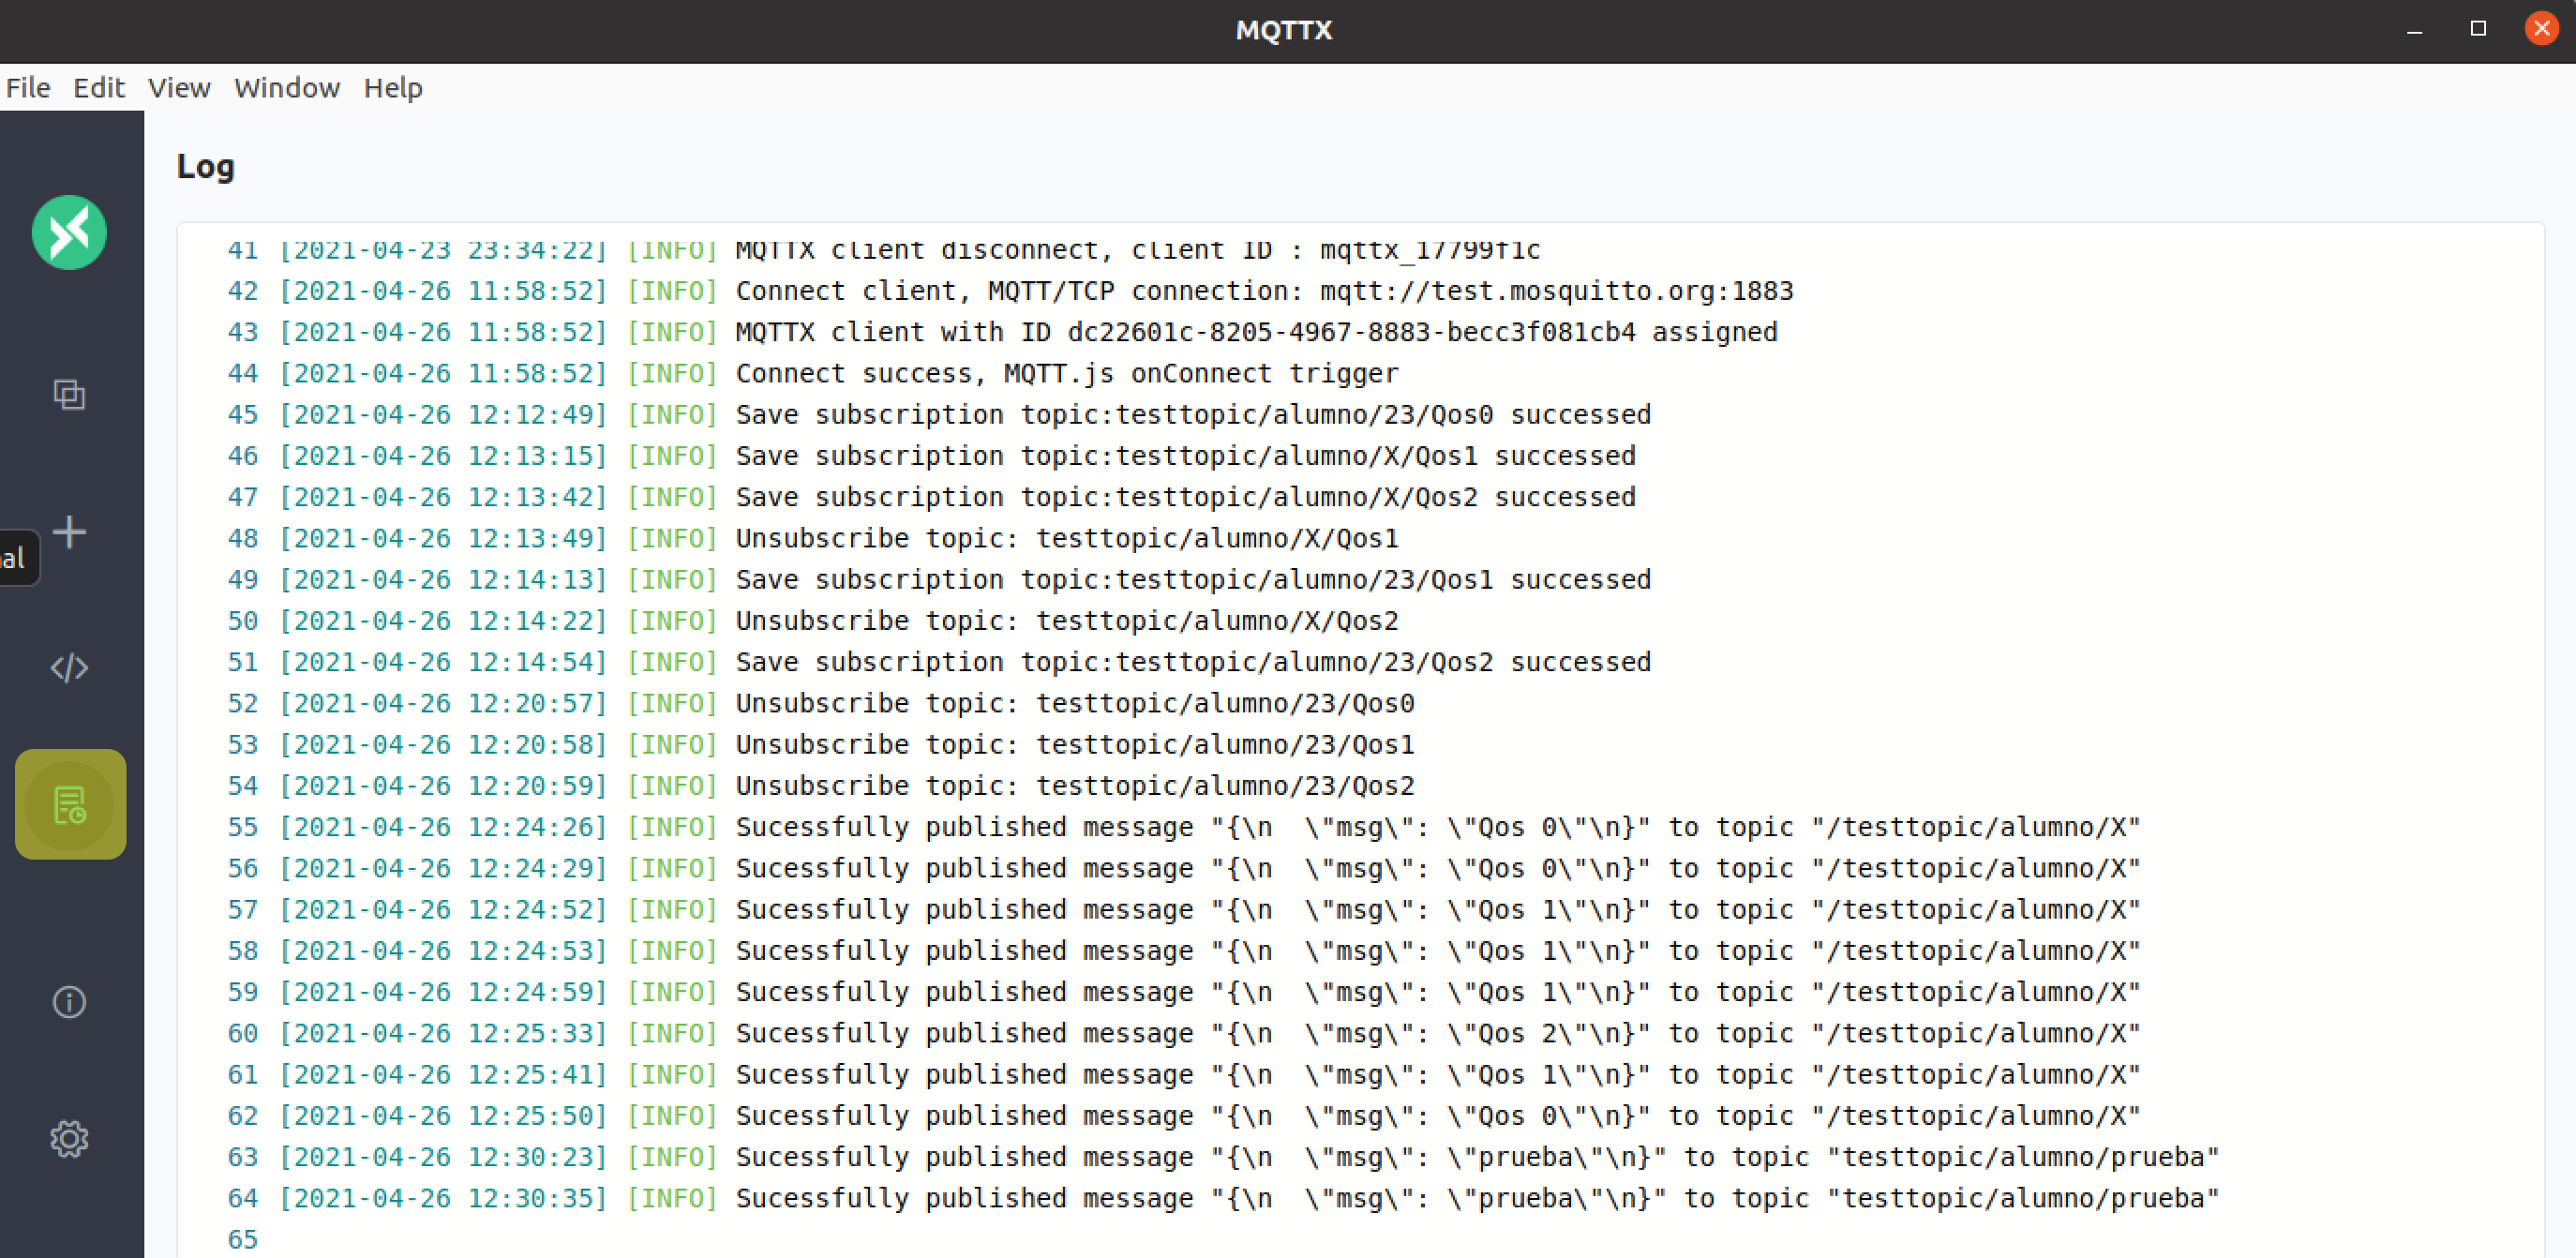
\includegraphics[width=0.8\textwidth]{enun16}
	\end{figure}
	\item Publica un mensaje con Qos 1 con el topic testtopic/p7/X. Incluye en el texto del mensaje
	Qos 1.
	\item Publica un mensaje con Qos 2 con el topic testtopic/p7/X. Incluye en el texto del mensaje
	Qos 2.
	\item Para la captura con Control+C.
	\item Abre la captura en wireshark Identifica los mensajes \textbf{Publish}
	\begin{figure}[H]
		\centering
		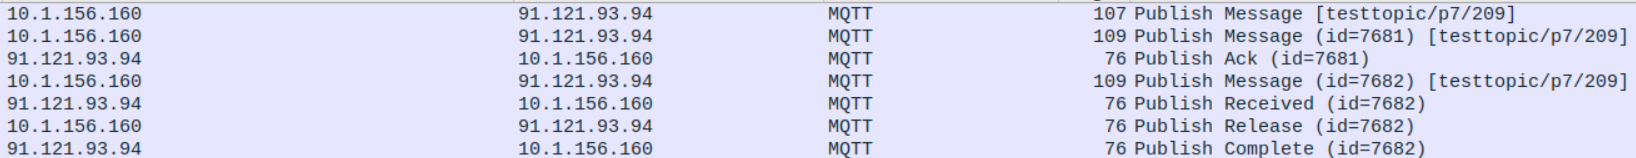
\includegraphics[width=0.8\textwidth]{ej7.8}
	\end{figure}
	\item Identifica el mensaje publicado por tu cliente como Qos = 0 ¿Cómo lo has reconocido? ¿Hay
	algún mensaje Publish Ack?\\
	Verifica tu suposición mirando también el contenido del mensaje.\\
	
	Lo he reconocido por el campo QoS level en la cabecera de MQTT.\\
	No hay ningún mensaje de Ack.
	\begin{figure}[H]
		\centering
		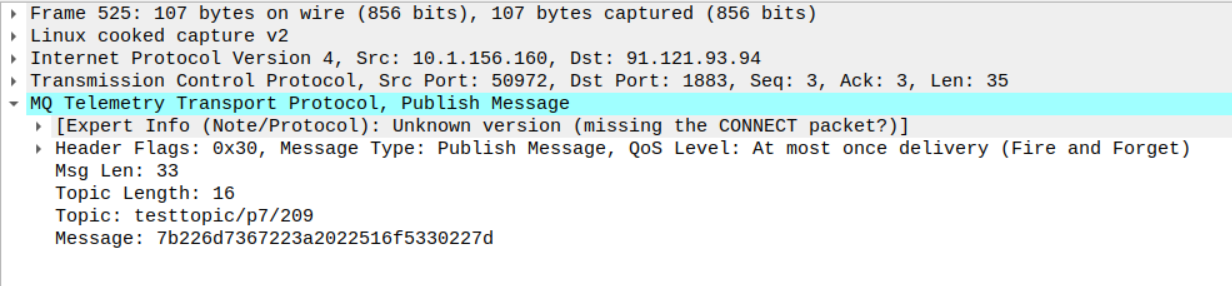
\includegraphics[width=0.8\textwidth]{ej7.9}
	\end{figure}
	\item Identifica el mensaje publicado por tu cliente como Qos = 1 ¿Cómo lo has reconocido? ¿Hay algún
	mensaje Publish Ack para el correspondiente Publish Request? ¿Cómo se hace la asociación entre
	el Publish Request y el Publish Ack?\\
	Verifica tu suposición mirando también el contenido del mensaje.\\
	
	Lo he reconocido por el campo QoS level en la cabecera de MQTT.\\
	Si que existen un mensaje Publish Ack, cuya asociación con el request es simplemente el identificador de mensaje que acepta el Ack.
	\begin{figure}[H]
		\centering
		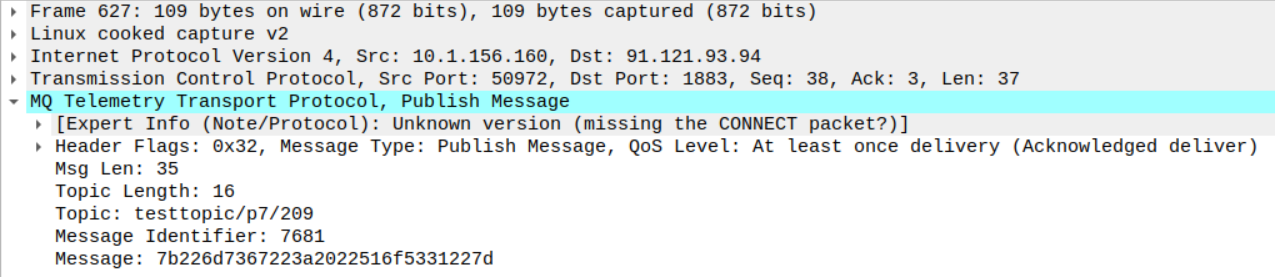
\includegraphics[width=0.8\textwidth]{ej7.10}
	\end{figure}
	\item Identifica el mensaje publicado Qos = 2 ¿Cómo lo has reconocido? ¿Hay algún mensaje Publish Ack para el correspondiente Publish Request? ¿Qué otros mensajes hay? ¿Cómo se hace la
	asociación entre el Publish Request y el Publish Ack? ¿Y con el Publish Release y Complete?\\
	
	Lo he reconocido por el campo QoS level en la cabecera de MQTT.\\
	No existe ningún un mensaje Publish Ack, sin embargo hay otros 3 mensajes.\\
	Para hacer la asociación entre el Request y el "Ack" el broker envía un Publish Received en vez del Ack. Cuando el cliente recive este mensaje lo confirma mandando de vuelta el Publish Release, y el broker vuelve a confirmar este mensaje con un Publish Complete.
	
\end{enumerate}
\chapter{Subscribe-Publish-Qos}
\section{Subscripción con Qos=0}
\begin{enumerate}
	\item Ponte a capturar tráfico en el fichero \textcolor{blue}{mqtt-05.cap}.
	\item Verifica que la conexión está activa.
	\item Subscribe tu cliente (consumidor) al siguiente tema con Qos=0, siendo X el número de tus
	direcciones IP:
	\begin{center}
		testtopic/p7/X/\#
	\end{center}
	\item Publica desde tu cliente (productor) un mensaje con Qos 0 con el topic testtopic/p7/X, siendo
	X tu el número de tus direcciones IP. Incluye en el texto del mensaje: Qos 0
	\item Publica un mensaje con Qos 1 con el topic testtopic/p7/X. Incluye en el texto del mensaje:
	Qos 1
	\item Publica un mensaje con Qos 2 con el topic testtopic/p7/X. Incluye en el texto del mensaje;
	Qos 2
	\item Para la captura con Control+C.
	\item Abre la captura en wireshark. \textbf{NOTA: Ten en cuenta que al transmitirse los mensajes
		de MQTT dentro de una conexión TCP puede haber varios mensajes MQTT dentro
		del mismo paquete capturado}.
	\item Verifica en el correspondiente mensaje MQTT que la subscripción hecha tiene un Qos=0. ¿Dónde
	lo has identificado?\\
	
	Lo he identificado en el campo Requested QoS.
	\begin{figure}[H]
		\centering
		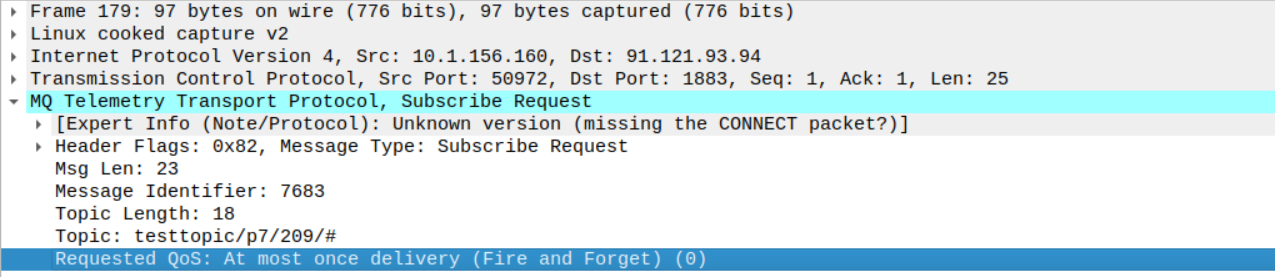
\includegraphics[width=0.8\textwidth]{ej8.1.9}
	\end{figure}
	\item Identifica los mensajes Publish enviados por el cliente y los enviados por el broker. ¿Cómo los
	has reconocido?\\
	
	Los mensajes que envia el broker serán los que compartan la Ip de origen con el que envía el Ack o con el que el puerto de origen sea 1883.
	\item Para el caso especifico del mensaje publicado por tu cliente (productor) con un Qos=0, ¿qué
	mensajes de tipo Publish se envían del cliente (productor del mensaje) al broker? ¿Qué mensajes
	de tipo Publish se transmiten desde el broker a tu cliente (consumidor)?\\
	
	Se envía un mensaje de tipo Message desde el cliente y otro desde el broker
	\item Para el caso especifico del mensaje publicado por tu cliente (productor) con un Qos=1, ¿qué
	mensajes de tipo Publish se envían del cliente (productor del mensaje) al broker? ¿Qué mensajes
	de tipo Publish se transmiten desde el broker a tu cliente (consumidor)? ¿Hay algún mensaje
	Publish Ack (cuántos)? ¿En qué momento temporal se transmite el mensaje de Publish desde el
	broker al consumidor (antes o después del mensaje Publish Ack)?\\
	
	Se envía un mensaje de tipo Message desde el cliente y el broker envía uno de tipo Message y otro de tipo Ack.\\
	El Publish Message se transmite antes del Ack.
	\item Para el caso especifico del mensaje publicado por tu cliente (productor) con un Qos=2, ¿qué
	mensajes de tipo Publish se envían del cliente (productor del mensaje) al broker? ¿Qué mensajes
	de tipo Publish se transmiten desde el broker a tu cliente (consumidor)? ¿Hay algún mensaje
	Publish Ack (cuántos)? ¿Después de qué mensaje se transmite el mensaje de Publish desde el
	broker al consumidor?\\
	
	El cliente envía un mensaje de tipo Message y otro de tipo Release ,y el broker transmite un mensaje de tipo Received, otro de Message y otro de Complete.\\
	No hay ningún mensaje de Ack, sin embargo hay un Received y un Complete.\\
	El mensaje de Publish Message lo envía el broker al recibir el mensaje de Release.
\end{enumerate}
\section{Subscripción con Qos=2}
\begin{enumerate}
	\item Ponte a capturar tráfico en el fichero \textcolor{blue}{mqtt-06.cap}.
	\item Verifica que la conexión está activa.
	\item \textbf{Elimina tu subscripción del cliente anterior}
	\item Subscribe tu cliente (consumidor) al siguiente tema con Qos=2
	\begin{center}
		testtopic/p7/X/\#
	\end{center}
	\item Publica desde tu cliente (productor) un mensaje con Qos 0 con el topic testtopic/p7/X. Incluye
	en el texto del mensaje: Qos 0
	\item Publica un mensaje con Qos 1 con el topic testtopic/p7/X. Incluye en el texto del mensaje:
	Qos 1
	\item Publica un mensaje con Qos 2 con el topic testtopic/p7/X. Incluye en el texto del mensaje:
	Qos 2
	\item Para la captura con Control+C.
	\item Abre la captura en wireshark.
	\item Verifica en el correspondiente mensaje MQTT que la subscripción hecha tiene un Qos=2. ¿Cómo
	lo has identificado?\\
	
	Lo he identificado en el campo Requested QoS.
	\item Identifica los mensajes Publish enviados por el cliente y los enviados por el broker. ¿Cómo los
	has reconocido?\\
	
	Los mensajes que envia el broker serán los que compartan la Ip de origen con el que envía el Ack o con el que el puerto de origen sea 1883.
	
	\item Para el caso especifico del mensaje publicado por tu cliente (productor) con un Qos=0, ¿qué
	mensajes de tipo Publish se envían del cliente (productor del mensaje) al broker? ¿Qué mensajes
	de tipo Publish se transmiten desde el broker a tu cliente (consumidor)? ¿Observas algún mensaje
	Publish Complete? ¿Por qué?\\
	
	Se envía un mensaje de tipo Message desde el cliente y otro desde el broker.\\
	No hay ningún mensaje de Publish Complete porque el cliente cuando lo publica tiene QoS 0, y cuando recibe el mensaje la QoS del mensaje recibido sigue siendo 0, por lo tanto no necesita hacer el Complete o el Ack.

	\item Para el caso especifico del mensaje publicado por tu cliente (productor) con un Qos=1, ¿qué
	mensajes de tipo Publish se envían del cliente (productor del mensaje) al broker? ¿Qué mensajes
	de tipo Publish se transmiten desde el broker a tu cliente (consumidor)? ¿Hay algún mensaje
	Publish Ack (cuántos)? ¿En qué momento temporal se transmite el mensaje de Publish desde
	el broker al consumidor (antes o después del mensaje Publish Ack)? ¿Observas algún mensaje
	Publish Complete? ¿Por qué?\\
	
	El cliente envía un mensaje de tipo Message y otro de tipo Ack al igual que el broker.\\
	El mensaje es publicado por el broker antes del Ack.\\
	No hay ningún mensaje de Publish Complete porque el cliente cuando lo publica tiene QoS 1, y cuando recibe el mensaje la QoS del mensaje recibido sigue siendo 1, por lo tanto se trata el paquete por ambas partes como si todo fuera con QoS 1.
	\item Para el caso especifico del mensaje publicado por tu cliente (productor) con un Qos=2, ¿qué
	mensajes de tipo Publish se envían del cliente (productor del mensaje) al broker? ¿Qué mensajes
	de tipo Publish se transmiten desde el broker a tu cliente (consumidor)?\\
	
	Ambos envían mensajes de tipo Message, Release, Complete y Received, ya que tienen que tratar el paquete por ambas partes como QoS 2
\end{enumerate}
Compara el comportamiento de la subscripción con Qos=0 con el comportamiento de la subscripción
con Qos=2:
\begin{enumerate}
	\setcounter{enumi}{14}
	\item Para la subscripción de tipo Qos=0, ¿cual es la Qos desde el productor al broker para cada uno
	de los mensajes Publish generados (Qos (0,1,2))? ¿Cuál es la Qos desde el broker al consumidor
	para cada uno de los mensajes Publish generados (Qos (0,1,2)? ¿Cuál sería la Qos productor-consumidor en cada caso desde un punto vista global de la comunicación para cada uno de los
	mensajes Publish generados (Qos (0,1,2)?\\
	
	Desde el productor al broker serían: 0, 1 y 2\\
	Desde el broker al consumidor sería: 0, 0 y 0\\
	Por lo tanto el QoS global sería 0, 0 y 0.
	\item Para la subscripción de tipo Qos=2, ¿cual es la Qos desde el productor al broker para cada uno
	de los mensajes Publish generados (Qos (0,1,2))? ¿cuál es la Qos desde el broker al consumidor
	para cada uno de los mensajes Publish generados (Qos (0,1,2)? ¿Cuál sería la Qos productor-consumidor en cada caso desde un punto vista global de la comunicación para cada uno de los
	mensajes Publish generados (Qos (0,1,2)?\\
	
	Desde el productor al broker serían: 0, 1 y 2\\
	Desde el broker al consumidor sería: 2, 2 y 2\\
	Por lo tanto el QoS global sería 0, 1 y 2.
\end{enumerate}
\chapter{Retain}
\begin{enumerate}
	\item Ponte a capturar tráfico en el fichero \textcolor{blue}{mqtt-07.cap}.
	\item Verifica que la conexión está activa.
	\item Publica un mensaje con el topic testtopic/p7/X y Retain Activado con el Qos=0. Incluye en el
	texto del mensaje: Retain1
	\begin{figure}[H]
		\centering
		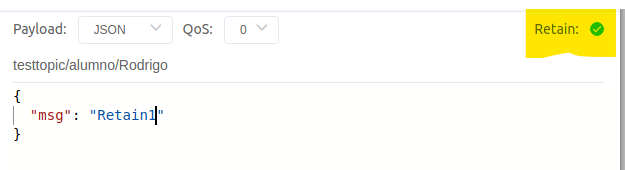
\includegraphics[width=0.8\textwidth]{enun17}
	\end{figure}
	\item Publica un mensaje en el topic testtopic/p7/X y Retain Activado con el Qos=0. Incluye en el
	texto del mensaje: Retain2
	\item Publica un mensaje en el topic testtopic/p7/X y Retain Desaactivado con el Qos=0. Incluye
	en el texto del mensaje: Retain3
	\item Desconecta la conexión.
	\begin{figure}[H]
		\centering
		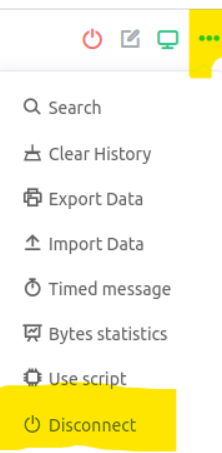
\includegraphics[width=0.15\textwidth]{enun18}
	\end{figure}
	\item Conéctate de nuevo
	\item Subscríbete al mismo topic de antes: testtopic/p7/\#
	\item Para la captura con Control+C.
	\item Abre la captura en wireshark. Identifica el mensaje Disconnect
	\begin{figure}[H]
		\centering
		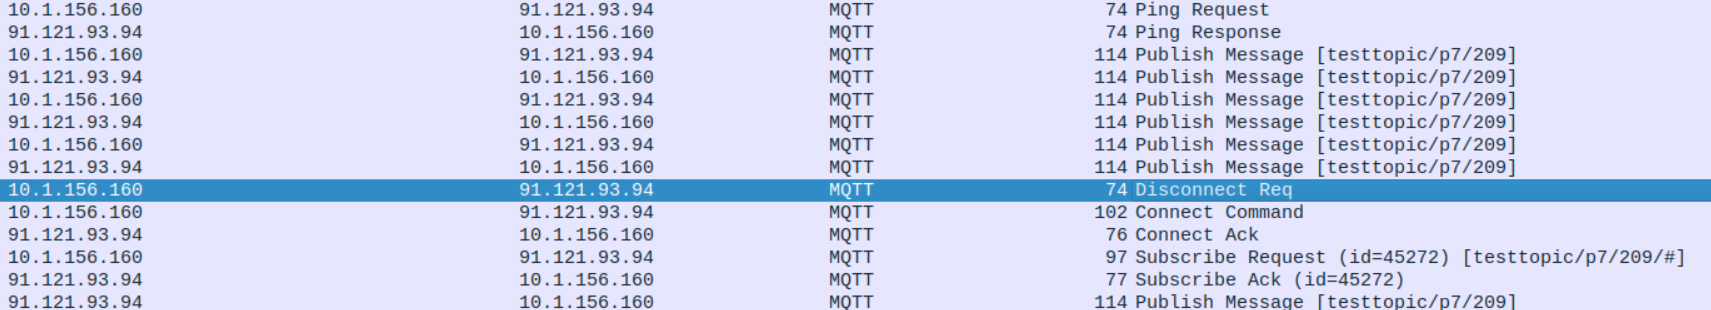
\includegraphics[width=0.8\textwidth]{ej9.10}
	\end{figure}
	\item ¿Qué longitud tiene el mensaje?\\
	
	Tiene longitud 0.
	\item Identifica los mensajes que tienen el flag Retain en su cabecera Retain. ¿Qué mensajes son?\\
	
	Son los siguientes mensajes
	\begin{figure}[H]
		\centering
		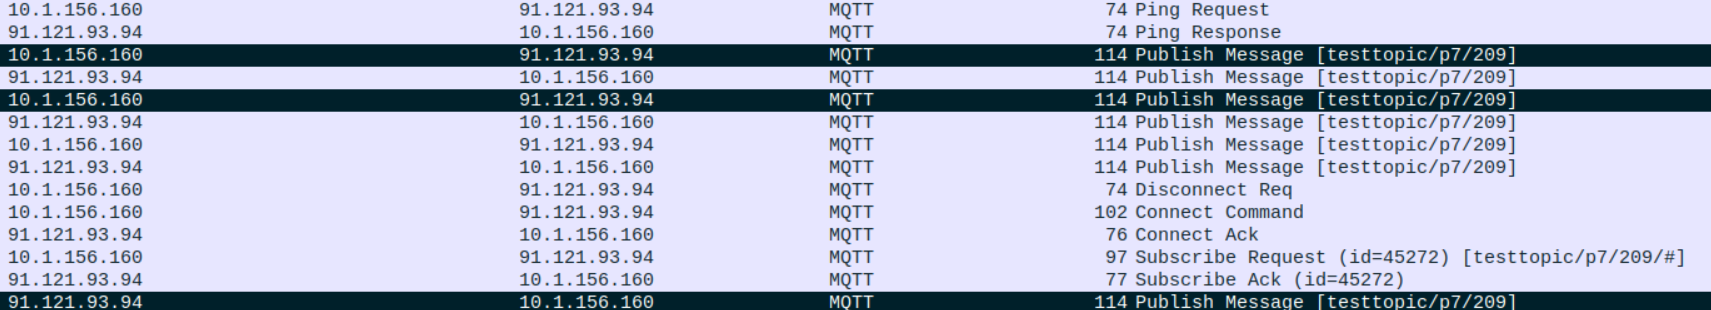
\includegraphics[width=0.8\textwidth]{ej9.12}
	\end{figure}
	\item ¿Qué texto de mensaje se recibe en el consumidor una vez que se vuelves a subscribir al topic
	testtopic/p7?\\
	
	El mensaje de Retain2 porque es el último.
	\item Ponte a capturar tráfico en el fichero \textcolor{blue}{mqtt-08.cap}.
	\item Verifica que la conexión está activa.
	\item Publica un mensaje (como productor) con el topic testtopic/p7/X y Retain Activado y Qos=2.
	Incluye en el texto del mensaje Retain3 Qos2
	\item Desconecta la conexión.
	\item Conéctate de nuevo
	\item Subscríbete al mismo topic de antes pero con Qos=2.
	\item Para la captura con Control+C.
	\item Abre la captura en wireshark.
	\item ¿Cuántos mensajes Publish Message se envían con el flag retain activo? ¿Son los mensajes publicados por la misma IP? ¿Puedes identificar qué IP tiene el broker y cuál el cliente?\\
	
	Se envían 3 mensajes con el flag activo, el primero proviene del cliente (cuando publicamos el mensaje) y el resto del broker.
	\begin{figure}[H]
		\centering
		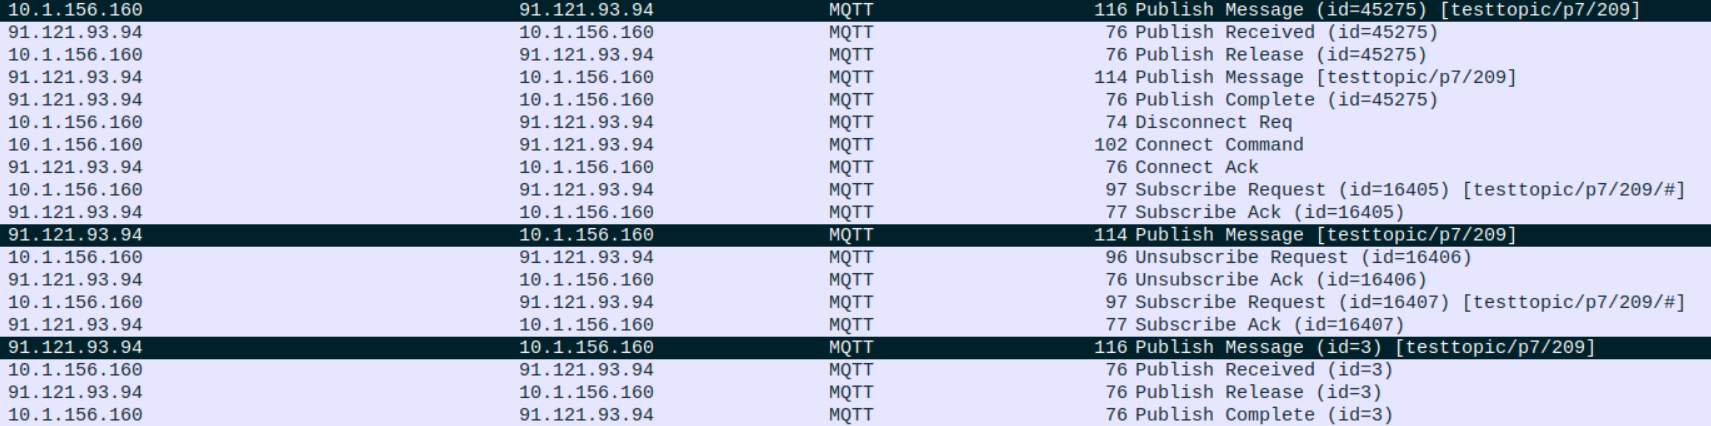
\includegraphics[width=0.8\textwidth]{ej9.22}
	\end{figure}
\end{enumerate}
\chapter{Unsubscribe}
\begin{enumerate}
	\item Ponte a capturar tráfico en el fichero \textcolor{blue}{mqtt-09.cap}.
	\item Verifica que la conexión está activa.
	\item Elimina la subscripción.
	\item Para la captura con Control+C.
	\item Abre la captura en wireshark. Identifica el mensaje Unsubscribe y Unsubscribe ACK
	\begin{figure}[H]
		\centering
		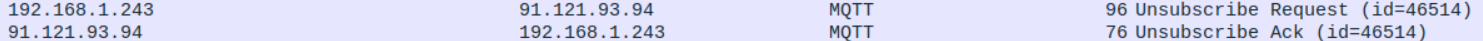
\includegraphics[width=0.8\textwidth]{ej10.5}
	\end{figure}
	\item ¿De qué topic estás quitando la subscripción?\\
	
	Del topic testtopic/p7/209/\#.
\end{enumerate}
\chapter{Last Will y Filtros de topic}
\begin{enumerate}
	\item Ponte a capturar tráfico en el fichero \textcolor{blue}{mqtt-10.cap}.
	\item Modifica la conexión para incluir los parámetro lastwill. Debes desconectar la conexión existente
	si esta activa.
	\begin{figure}[H]
		\centering
		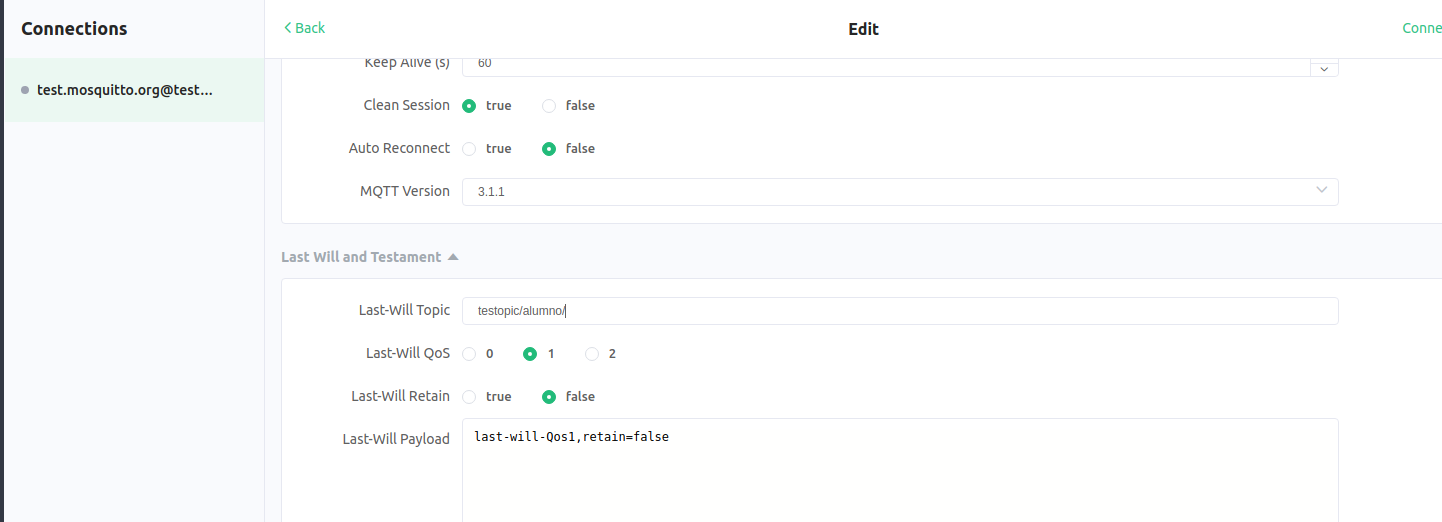
\includegraphics[width=0.8\textwidth]{enun19}
	\end{figure}
	\item Los parámetros son:
	\begin{flushleft}
		LastWillTopic=testtopic/p7/\\
		LastWill-Qos=1\\
		LastWill-Retain=False\\
		LastWill Message
	\end{flushleft}
	Incluid el siguiente mensaje: LastWillQos1,RetainFalse
	\item Verifica que la conexión está activa.
	\item Elimina cualquier subscripción que tengas
	\item Crea una subscripción testtopic/p7/X/+
	\item Publica el siguiente topic: testtopic/p7/X/aa/bb
	\item Publica el siguiente topic: testtopic/p7/X/aa
	\item ¿Cuántos mensajes se reciben por parte del consumidor? ¿Por qué?\\
	
	Solo 1 porque el comodín "+" hace que solo coincida un nivel de tema.
	\item Crea una subscripción testtopic/p7/X/\#
	\item Publica el siguiente topic testtopic/p7/X/aa/bb
	\item Publica el siguiente topic testtopic/p7/X/aa
	\item ¿Cuántos mensajes se reciben por parte del consumidor? ¿Por qué?\\
	
	Se reciben los 2 del nuevo subscriptor y 1 del anterior, porque el comodín del "\#" coincide con cualquier número de niveles dentro de un tema.
	\item Para la captura con Control+C.
	\item Abre la captura en wireshark
	\item ¿En qué mensaje puedes ver el parámetro LastWill? ¿Qué lastWillQos tiene?\\
	
	Solo se puede ver en el Connect y tiene un QoS de 1.
\end{enumerate}
\chapter{Persistencia sesión}
\begin{enumerate}
	\item Ponte a capturar tráfico creando el fichero \textcolor{blue}{mqtt-11.cap}.
	\item Modifica la conexión para conectar usando el parámetro \textbf{CleanSession activado (true)}
	\begin{figure}[H]
		\centering
		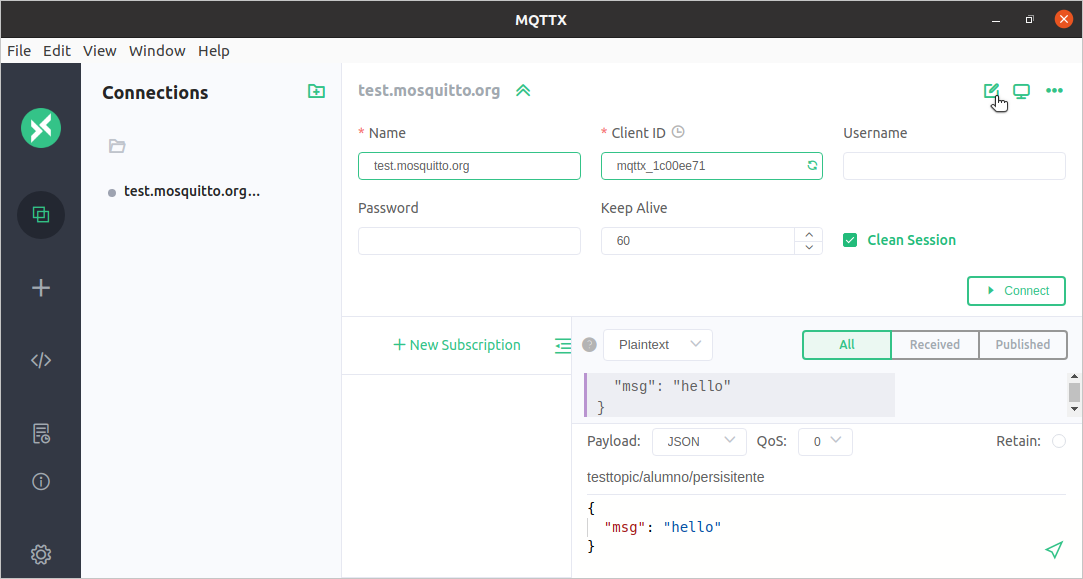
\includegraphics[width=0.8\textwidth]{enun20}
	\end{figure}
	\begin{figure}[H]
		\centering
		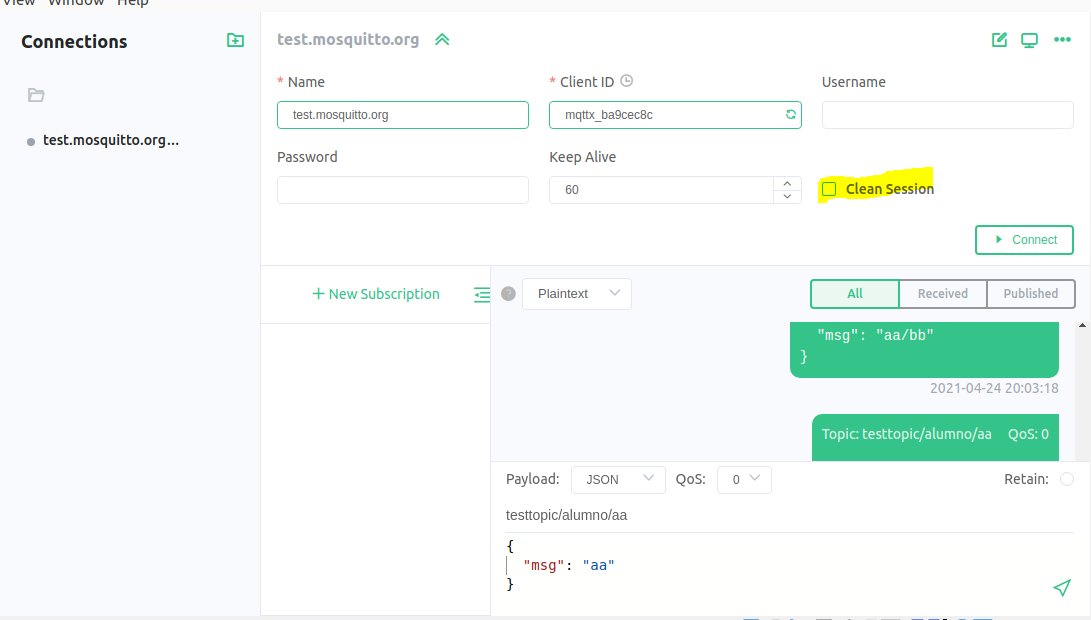
\includegraphics[width=0.8\textwidth]{enun21}
	\end{figure}
	\item Crea una subscripción testtopic/p7/X/\#
	\item Desconecta la sesión con el broker (servidor)
	\item Conectate de nuevo con el parámetro \textbf{Clean Session Activado}
	\item Publica el siguiente topic: testtopic/p7/X/ con Qos=2
	\item Desconecta la conexión con el broker (servidor)
	\item Modifica la conexión para conectar usando el parámetro \textbf{CleanFlag desactivado (false)}
	\item Crea una subscripción testtopic/p7/X/\#
	\item Desconecta la sesión con el broker (servidor)
	\item Conectate de nuevo con el parámetro \textbf{Clean Session desactivado}
	\item Publica el siguiente topic: testtopic/p7/X/ con Qos=2
	\item Desconecta la conexión
	\item Para la captura.
	\item Abre la captura en wireshark
	\item ¿En el cliente consumidor has recibido algún mensaje cuando el Clean Session estaba habilitado?
	¿y cuando estaba deshabilitado? ¿Por qué?\\
	
	Cuando estaba el flag activado no he recibido ningún mensaje porque al cerrar la sesión el subscriptor se ha desubscrito del topic.\\
	Mientras que cuando estaba deshabilitado he recibido los mensajes porque el subscriptor sigue conectado a ese topic.
\end{enumerate}
\end{document}